\documentclass[conference]{IEEEtran}
% Some Computer Society conferences also require the compsoc mode option,
% but others use the standard conference format.
%
% If IEEEtran.cls has not been installed into the LaTeX system files,
% manually specify the path to it like:
% \documentclass[conference]{../sty/IEEEtran}

% *** Do not adjust lengths that control margins, column widths, etc. ***
% *** Do not use packages that alter fonts (such as pslatex).         ***
% There should be no need to do such things with IEEEtran.cls V1.6 and later.
% (Unless specifically asked to do so by the journal or conference you plan
% to submit to, of course. )

\usepackage[utf8]{inputenc}
\usepackage[swedish]{babel}
\usepackage{hyperref}
\usepackage{graphicx}
\usepackage{caption}
\usepackage{listings}
\usepackage{color}

\renewcommand{\lstlistingname}{Kod}

\definecolor{dkgreen}{rgb}{0,0.6,0}
\definecolor{gray}{rgb}{0.5,0.5,0.5}
\definecolor{mauve}{rgb}{0.58,0,0.82}

\lstdefinelanguage{JavaScript}{
  keywords={break, case, catch, continue, debugger, default, delete, do, else, finally, for, function, if, in, instanceof, new, return, switch, this, throw, try, typeof, var, void, while, with},
  morecomment=[l]{//},
  morecomment=[s]{/*}{*/},
  morestring=[b]',
  morestring=[b]",
  sensitive=true
}
\lstdefinelanguage{GLSL}
{
sensitive=true,
morekeywords=[1]{
attribute, const, uniform, varying,
layout, centroid, flat, smooth,
noperspective, break, continue, do,
for, while, switch, case, default, if,
else, in, out, inout, float, int, void,
bool, true, false, invariant, discard,
return, mat2, mat3, mat4, mat2x2, mat2x3,
mat2x4, mat3x2, mat3x3, mat3x4, mat4x2,
mat4x3, mat4x4, vec2, vec3, vec4, ivec2,
ivec3, ivec4, bvec2, bvec3, bvec4, uint,
uvec2, uvec3, uvec4, lowp, mediump, highp,
precision, sampler1D, sampler2D, sampler3D,
samplerCube, sampler1DShadow,
sampler2DShadow, samplerCubeShadow,
sampler1DArray, sampler2DArray,
sampler1DArrayShadow, sampler2DArrayShadow,
isampler1D, isampler2D, isampler3D,
isamplerCube, isampler1DArray,
isampler2DArray, usampler1D, usampler2D,
usampler3D, usamplerCube, usampler1DArray,
usampler2DArray, sampler2DRect,
sampler2DRectShadow, isampler2DRect,
usampler2DRect, samplerBuffer,
isamplerBuffer, usamplerBuffer, sampler2DMS,
isampler2DMS, usampler2DMS,
sampler2DMSArray, isampler2DMSArray,
usampler2DMSArray, struct},
morekeywords=[2]{
radians,degrees,sin,cos,tan,asin,acos,atan,
atan,sinh,cosh,tanh,asinh,acosh,atanh,pow,
exp,log,exp2,log2,sqrt,inversesqrt,abs,sign,
floor,trunc,round,roundEven,ceil,fract,mod,modf,
min,max,clamp,mix,step,smoothstep,isnan,isinf,
floatBitsToInt,floatBitsToUint,intBitsToFloat,
uintBitsToFloat,length,distance,dot,cross,
normalize,faceforward,reflect,refract,
matrixCompMult,outerProduct,transpose,
determinant,inverse,lessThan,lessThanEqual,
greaterThan,greaterThanEqual,equal,notEqual,
any,all,not,textureSize,texture,textureProj,
textureLod,textureOffset,texelFetch,
texelFetchOffset,textureProjOffset,
textureLodOffset,textureProjLod,
textureProjLodOffset,textureGrad,
textureGradOffset,textureProjGrad,
textureProjGradOffset,texture1D,texture1DProj,
texture1DProjLod,texture2D,texture2DProj,
texture2DLod,texture2DProjLod,texture3D,
texture3DProj,texture3DLod,texture3DProjLod,
textureCube,textureCubeLod,shadow1D,shadow2D,
shadow1DProj,shadow2DProj,shadow1DLod,
shadow2DLod,shadow1DProjLod,shadow2DProjLod,
dFdx,dFdy,fwidth,noise1,noise2,noise3,noise4,
EmitVertex,EndPrimitive},
morekeywords=[3]{
gl_VertexID,gl_InstanceID,gl_Position,
gl_PointSize,gl_ClipDistance,gl_PerVertex,
gl_Layer,gl_ClipVertex,gl_FragCoord,
gl_FrontFacing,gl_ClipDistance,gl_FragColor,
gl_FragData,gl_MaxDrawBuffers,gl_FragDepth,
gl_PointCoord,gl_PrimitiveID,
gl_MaxVertexAttribs,gl_MaxVertexUniformComponents,
gl_MaxVaryingFloats,gl_MaxVaryingComponents,
gl_MaxVertexOutputComponents,
gl_MaxGeometryInputComponents,
gl_MaxGeometryOutputComponents,
gl_MaxFragmentInputComponents,
gl_MaxVertexTextureImageUnits,
gl_MaxCombinedTextureImageUnits,
gl_MaxTextureImageUnits,
gl_MaxFragmentUniformComponents,
gl_MaxDrawBuffers,gl_MaxClipDistances,
gl_MaxGeometryTextureImageUnits,
gl_MaxGeometryOutputVertices,
gl_MaxGeometryOutputVertices,
gl_MaxGeometryTotalOutputComponents,
gl_MaxGeometryUniformComponents,
gl_MaxGeometryVaryingComponents,gl_DepthRange},
morecomment=[l]{//},
morecomment=[s]{/*}{*/},
morecomment=[l][keywordstyle4]{\#},
}

\lstset{frame=tb,
  language=JavaScript,
  aboveskip=3mm,
  belowskip=3mm,
  showstringspaces=false,
  columns=flexible,
  basicstyle={\small\ttfamily},
  numbers=none,
  numberstyle=\tiny\color{gray},
  keywordstyle=\color{blue},
  commentstyle=\color{dkgreen},
  stringstyle=\color{mauve},
  breaklines=true,
  breakatwhitespace=true,
  tabsize=2,
  numbers=left,
  xleftmargin=1.5em,
  framexleftmargin=1.5em
}

\newenvironment{Figure}
  {\par\medskip\noindent\minipage{\linewidth}}
  {\endminipage\par\medskip}

% correct bad hyphenation here
\hyphenation{op-tical net-works semi-conduc-tor}

\begin{document}
%
% paper title
% Titles are generally capitalized except for words such as a, an, and, as,
% at, but, by, for, in, nor, of, on, or, the, to and up, which are usually
% not capitalized unless they are the first or last word of the title.
% Linebreaks \\ can be used within to get better formatting as desired.
% Do not put math or special symbols in the title.
\title{My Little Planet}

% author names and affiliations
% use a multiple column layout for up to three different
% affiliations
\author{\IEEEauthorblockN{Klas Eskilson}
\IEEEauthorblockA{TNM084, Linköpings Universitet\\
klaes950@student.liu.se\\
\url{http://klaseskilson.se/TNM084-my-little-planet}}}

% make the title area
\maketitle

\lstset{language=JavaScript}

% As a general rule, do not put math, special symbols or citations
% in the abstract
\begin{abstract}
Denna rapport diskuterar teorin, implementationen och resultatet utav
procedurella brusfunktioner i ett WebGL-program. I programmet används flera shaders skrivna i GLSL för att skapa variation och animation över ytor med goda resultat ur ett prestandaperspektiv.
\end{abstract}

% no keywords

\section{Introduktion}

Både webben och datorgrafik är två områden i ständig utveckling. Starkare och mer avancerade tekniker blir tillgängliga i webbläsare, medan utvecklingen inom datorgrafiken möjliggör allt mer avancerade visualiseringar och program. Kombinationen av dessa två tekniker möts i WebGL, där en förenklad version av grafikbiblioteket OpenGL är tillgänglig. Detta gör det möjligt att skapa avancerad datorgrafik i webbläsare på flera olika sorters enheter, såväl datorer som mobila enheter \cite{ref:caniuse}.

I programmet som tas upp i denna rapport har flera olika varianter av så kallat procedurellt brus använts. Att använda procedurella metoder för bilder innebär att använda matematiska funktioner för att exempelvis skapa en textur eller varians över en yta. Att använda procedurellt brus som i denna rapport är således att skapa variation som lätt kan uppfattas som slumpartat, när den egentligen inte är det.

\section{Teori}

Brusfunktionerna som använts är dels \emph{simplex}-brus och dels vad som kallas klassiskt Perlin-brus. Simplex-metoderna är skrivna av I.~McEwan på Ashima Arts och de klassiska Perlin-brusfunktionerna är skrivna av S.~Gustavsson på Linköpings Universitet.

Perlin-brus fungerar så att punkter över en linje, plan, volym eller motsvarande form beroende på antalet dimensioner som använts ges en pseudo-slumpartad lutning. Punkterna mellan dessa fasta punkter interpoleras sedan mjukt. \cite{ref:stegu}

Simplex-bruset är betydligt mer avancerat, men har fördelarna att högre dimensioner inte nödvändigtvis påverkar prestandan lika negativt som dimensionsökning i Perlin-brus kan göra. För en förklaring av dessa metoder hänvisas till S.~Gustavssons artikel \emph{Simplex noise demystified} \cite{ref:stegu}. Kortfattat fungerar simplex-brus så att den enklast möjliga formen för varje dimension skapas så att den om den upprepades skulle kunna fylla hela rymden. Detta ger en kropp, eller motsvarande beroende på dimension, som har så få hörn som möjligt, $N + 1$ hörn om rymden har $N$ dimensioner. Varje hörn påverkas sedan av, och endast av, sina närmaste grannar, vilket underlättar vid interpolationen. Detta leder till att Perlin-brus inte lider av att användas i högre dimensioner. \cite{ref:stegu}

\section{Implementation}

\begin{Figure}
  \centering
    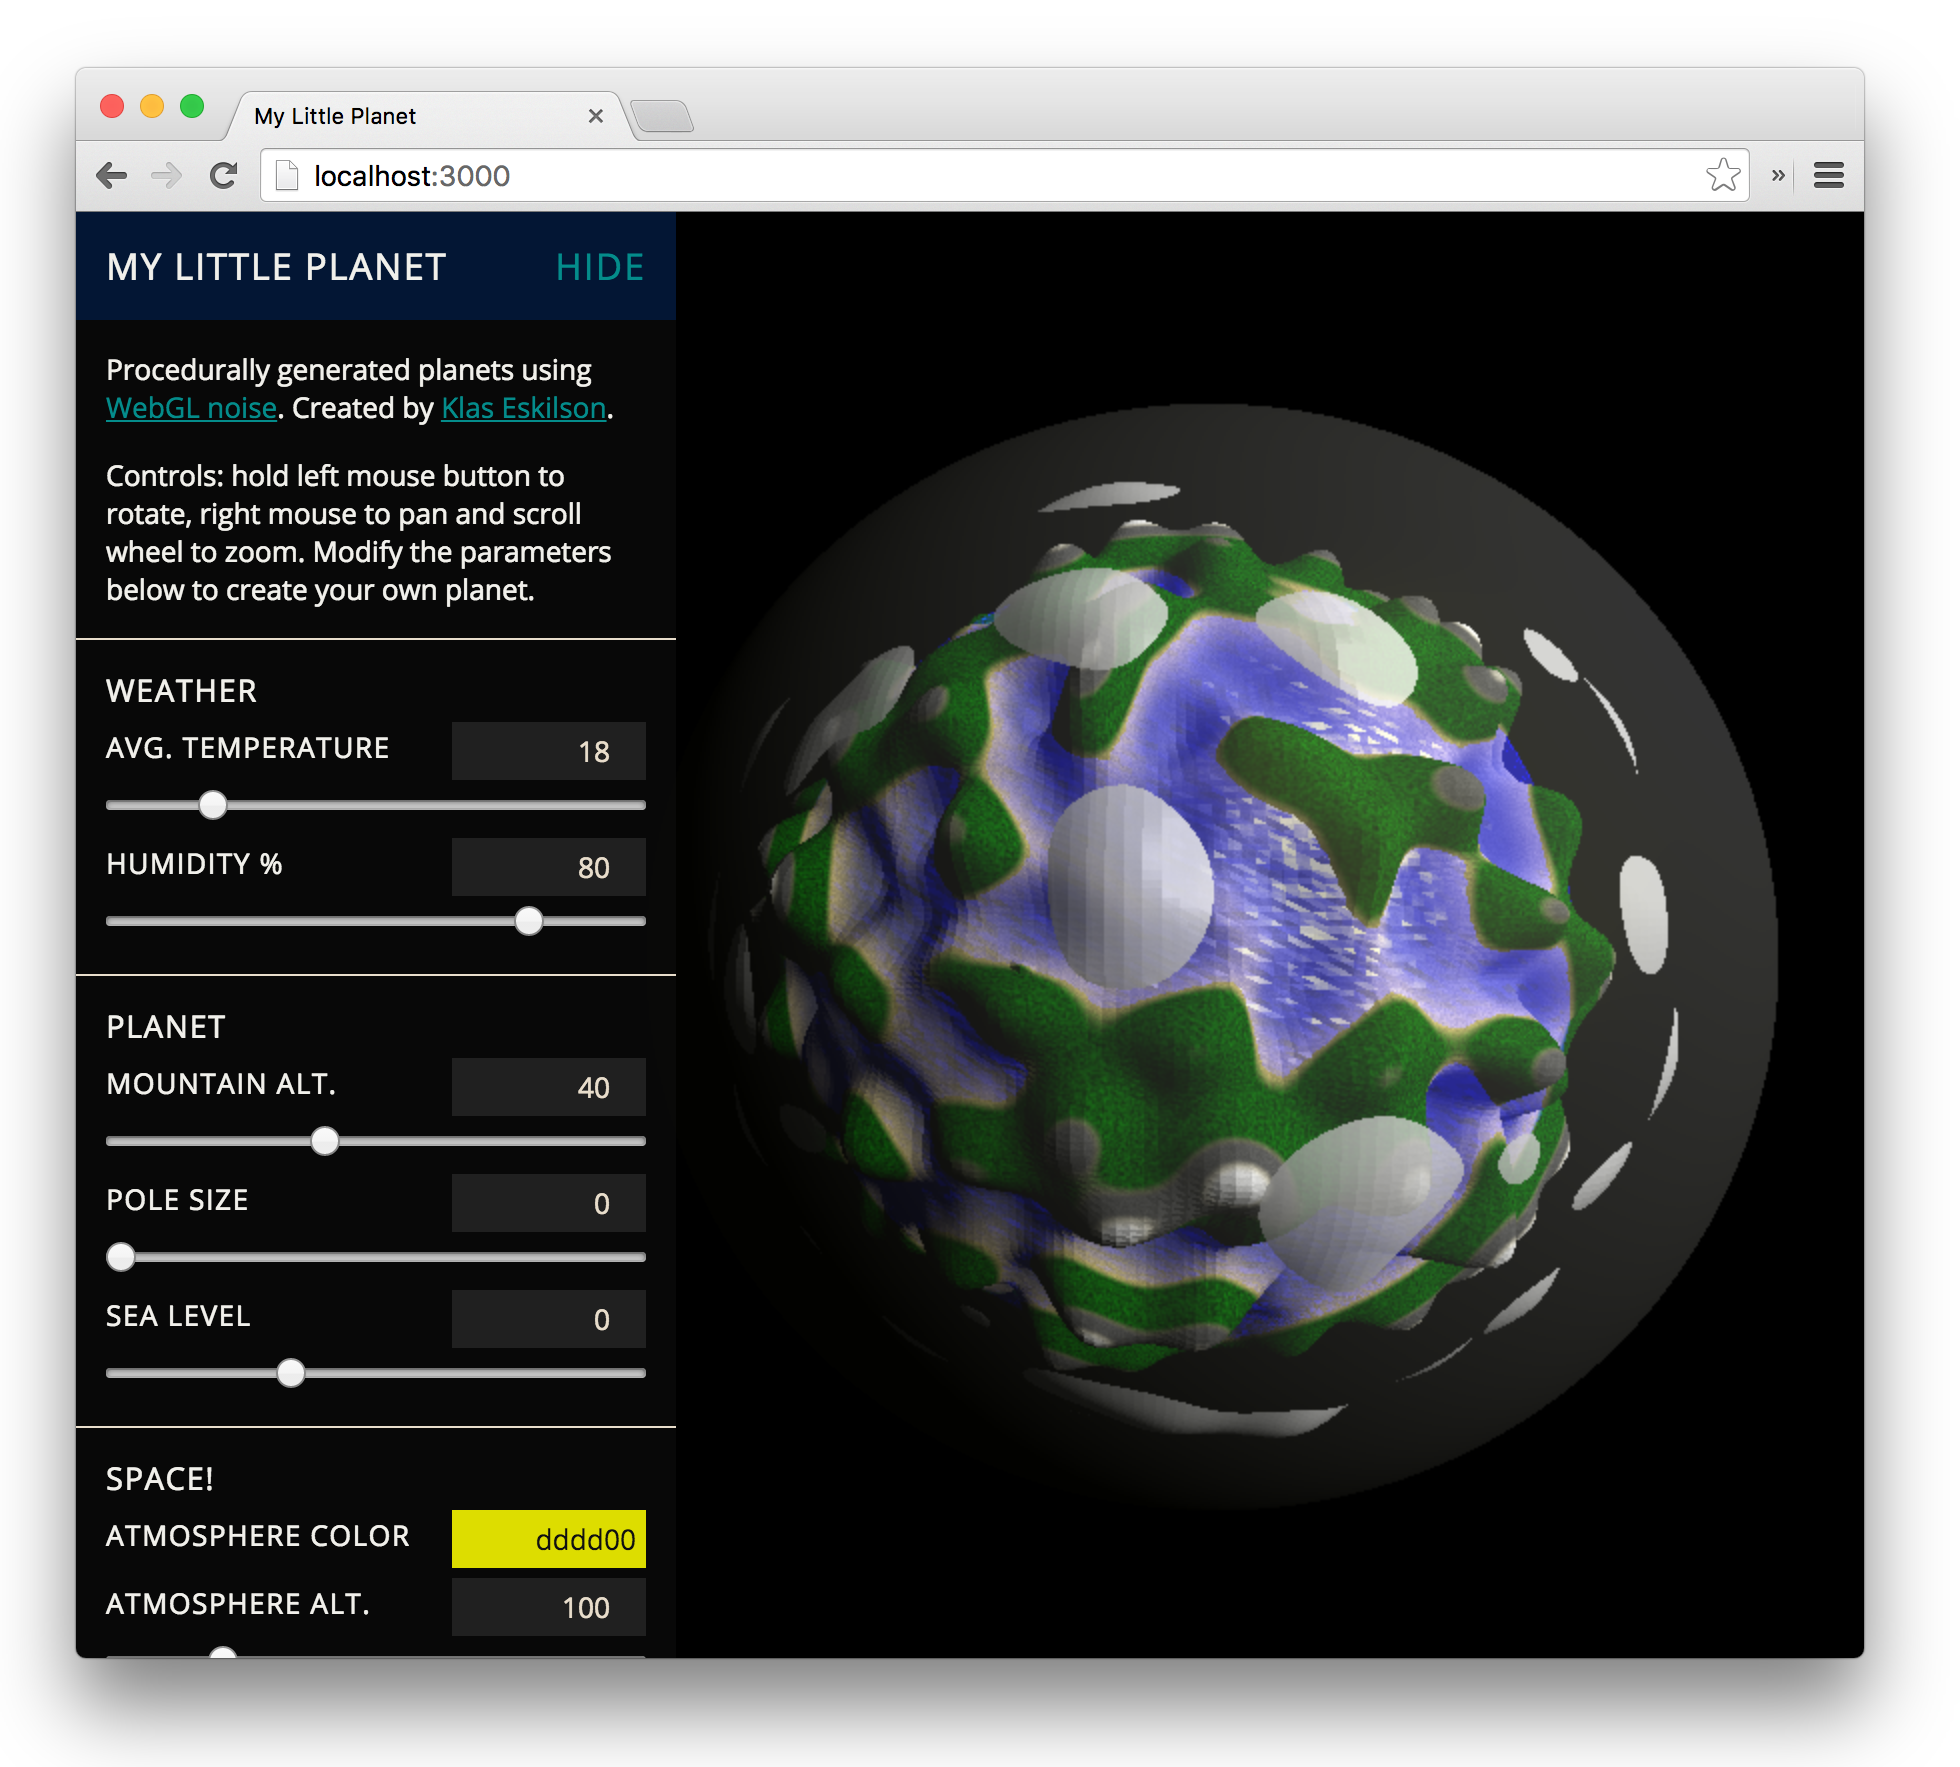
\includegraphics[width=\linewidth]{./images/app}
  \captionof{figure}{Det färdiga programmet.}\label{fig:app}
\end{Figure}

Programmet är skrivet i Javascriptramverket Three.JS, vars mål är att förenkla skapandet av WebGL-program i 3D. I scenen renderas fyra sfärer för planeten; en för ytan, en för vattnet, en för molnen samt en för atmosfären. Dessa har egna \emph{vertex-} samt \emph{fragmentshaders}. Även en enkel sfär som representerar ljuskällan renderas.

\subsection{Ytvariation samt -animation}

För jordytan har tredimensionellt brus applicerat för att skapa toppar och dalar. Vertex-punkterna har förskjutits längs med normalen till punkten. Detta skapar en kontirnuelig förändring över ytan. För att skapa olika miljöer på planeten används denna förskjutning till att bestämma punktes höjd, varpå olika färger applicerats på olika höjd. I ordning från högst till lägst: snö, berg, skog, sand, berg. Fyrdimensionellt brus användes på vatten- samt molnytan för att låta dessa variera även över tid.

För att skapa en planetyta som ser så trovärdig ut som möjligt applicerades brus med nio oktaver utöver grundbruset. Detta gjordes i en loop på vertexshadern där brusfunktionens effekt minskade i takt med att dess variation ökade. Detta leder till att det blir variationer med olika storlekar över ytan.

\begin{lstlisting}[language=GLSL,caption=Uträkning av höjdförändringen för planetytan (GLSL),label={lst:elevation}]
float elevation = 0.0;
for (float i = 1.0; i < 10.0; i += 1.0) {
  elevation += (1.0 / i)
      * snoise(i * position);
}
\end{lstlisting}

\subsection{Ljussättning}

Samtliga ytor gavs en Phong-reflektans med ambient, diffus och spekulär del. För att ljussättningen skulle fungera korrekt trots att vertex-punkterna förflyttats måste även normalerna uppdateras. Detta innebar ett problem då varken vertex- eller fragmentshadern inte vet om vilka punkter som ligger omkring den aktuella punkten. Varje förskjutning längs med normalen behandlas därför helt individuellt, ovetande om hur den förskjutning ställs i relation till de omkringliggande punkterna och hur detta påverkar punktens lutning. För att lösa detta användes \emph{GLSL}s funktioner \texttt{dFdx} samt \texttt{dFdy} i fragmentshadern. Dessa funktioner kan beräkna en punkts lokala derivata i x- respektive y-led. Normalen ges sedan av kryssprodukten mellan dessa två vektorer, se ekvation \ref{eq:normal}.

\begin{equation}
  \overrightarrow{n} = \overrightarrow{dFdx} \times \overrightarrow{dFdy}
  \label{eq:normal}
\end{equation}

\texttt{dFdx} och \texttt{dFdy} fungerar som så att fragmentshadern hanterar upp bildpunkterna i grupper om fyra, så kallade \emph{quads}, i en grupp av trådar på grafikkortet. Dessa punkter utgör tillsammans en kvadrat, och det är inom denna kvadrat som derivatorna i x- och y-led räknas ut genom att varje tråd på grafikkortet hämtar de omkringliggande trådarnas motsvarande värde. Se kod \ref{lst:dfdx} för implementation. \cite{ref:dfdx}

\begin{lstlisting}[language=GLSL,caption=Uträkning av ny normal (GLSL),label={lst:dfdx}]
vec3 dx = dFdx(position);
vec3 dy = dFdy(position);
vec3 newNormal = normalize(cross(dx, dy));
\end{lstlisting}

\subsection{Gränssnitt}

\begin{Figure}
  \centering
    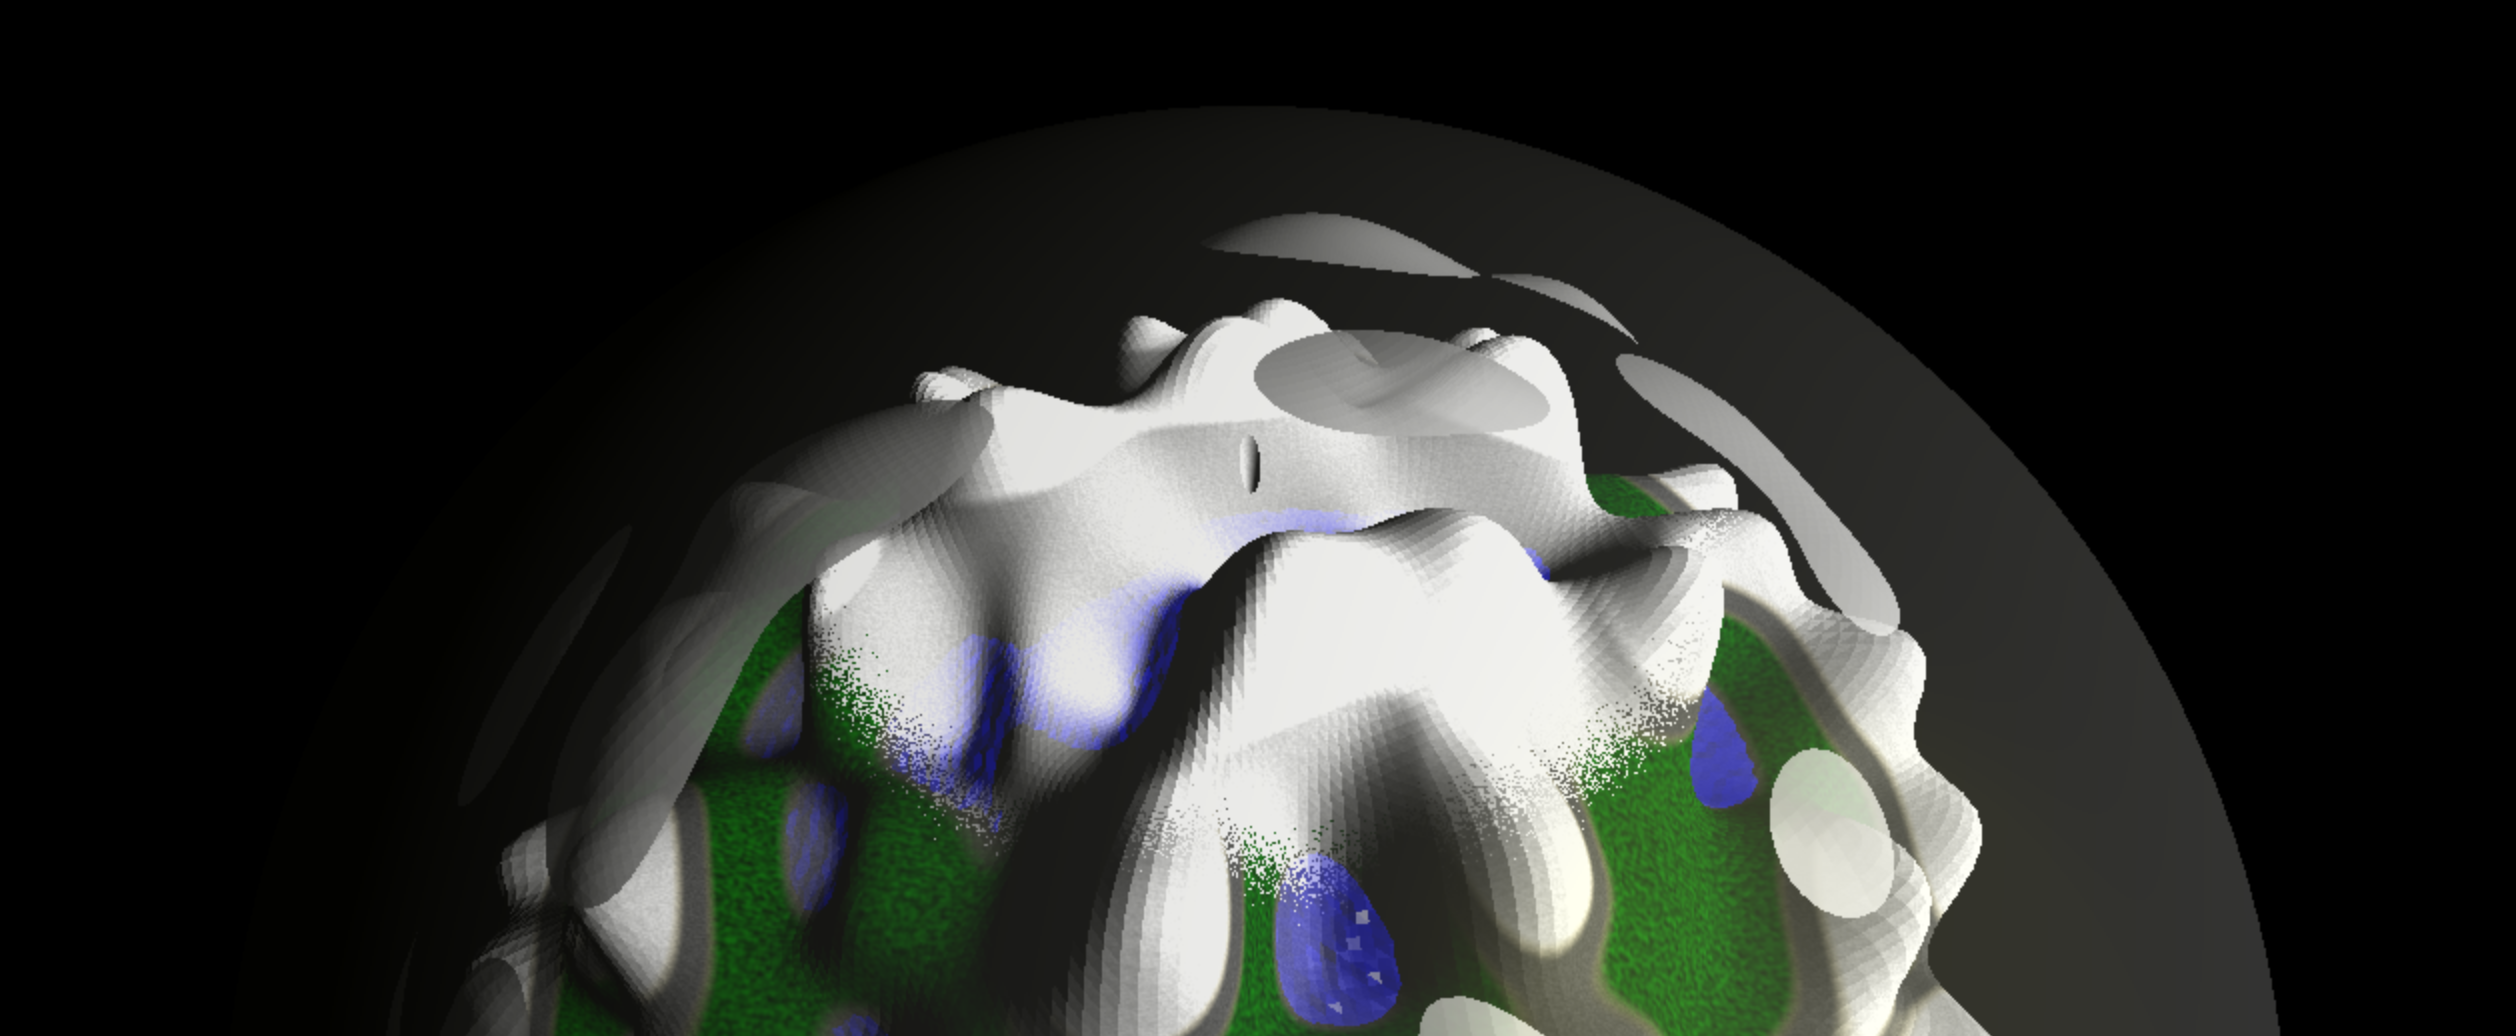
\includegraphics[width=0.9\linewidth]{./images/poles}
  \captionof{figure}{Detaljbild av planet med ökad polstorlek samt sänkt vattennivå.}\label{fig:poles}
\end{Figure}

För att göra programmet mer intressant för användaren skapades ett enkelt gränssnitt. Här kan användaren kontrollera en mängd parametrar som styr planetens utseende. Ett urval är polernas storlek, bergens höjd, molnens täthet och atmosfärens spekulära reflektionsfärg. Det går även att styra mer abstrakta parametrar såsom medeltemperatur och luftfuktighet, vilka i sin tur styr andra parametrar. I figur \ref{fig:poles} och \ref{fig:big} ses planeter där några parametrar ändrats. I figur \ref{fig:default} ses en planet med standardinställningarna.

\begin{Figure}
  \centering
    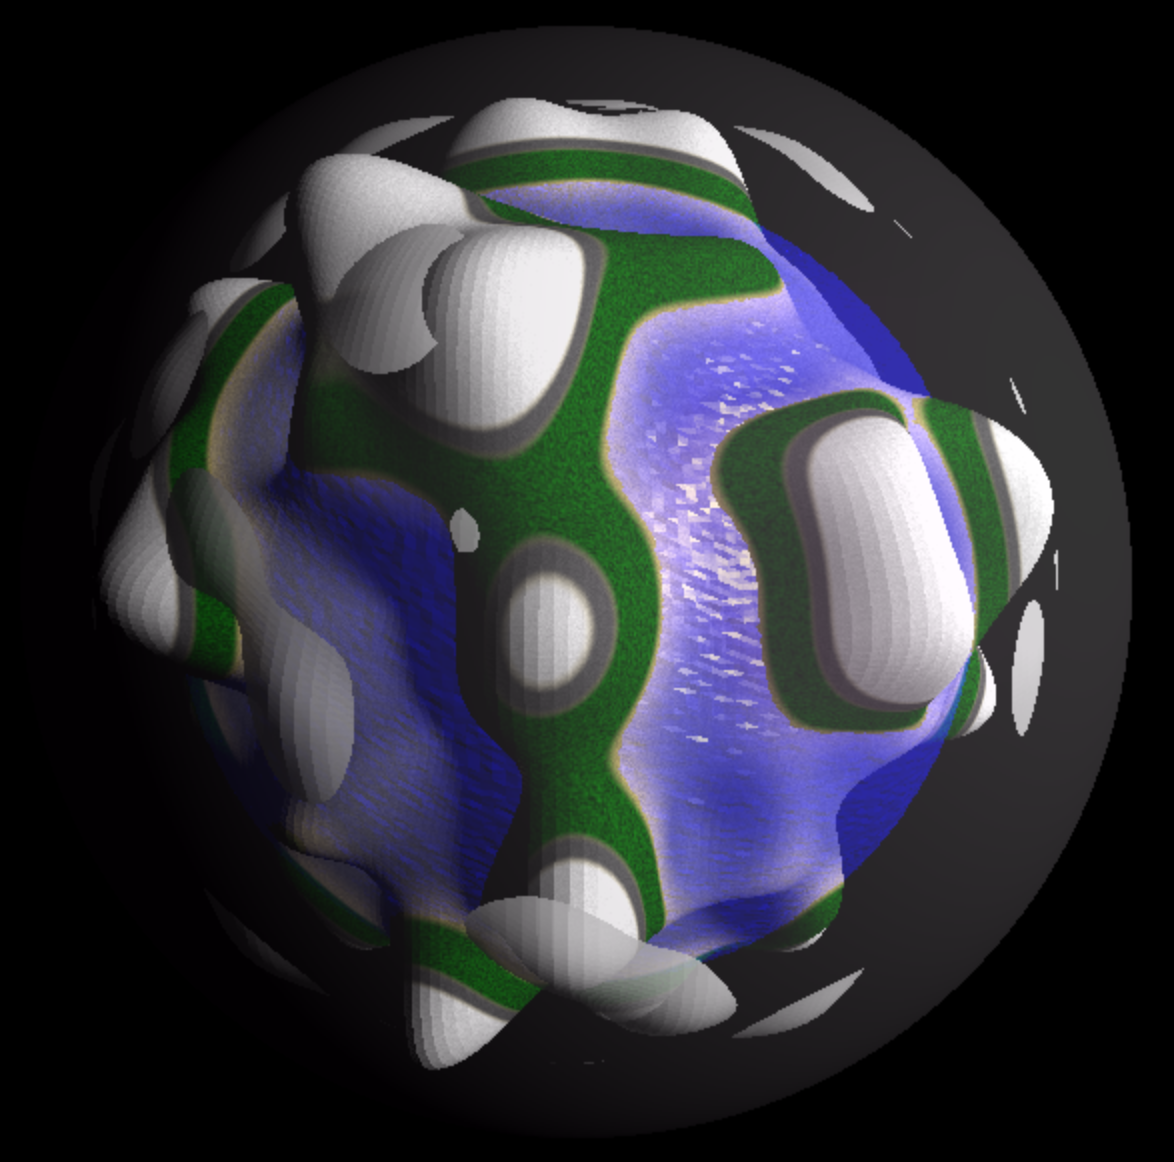
\includegraphics[width=0.8\linewidth]{./images/bigger}
  \captionof{figure}{Planet med sänkt ytvariation samt ökad bergshöjd.}\label{fig:big}
\end{Figure}

\begin{Figure}
  \centering
    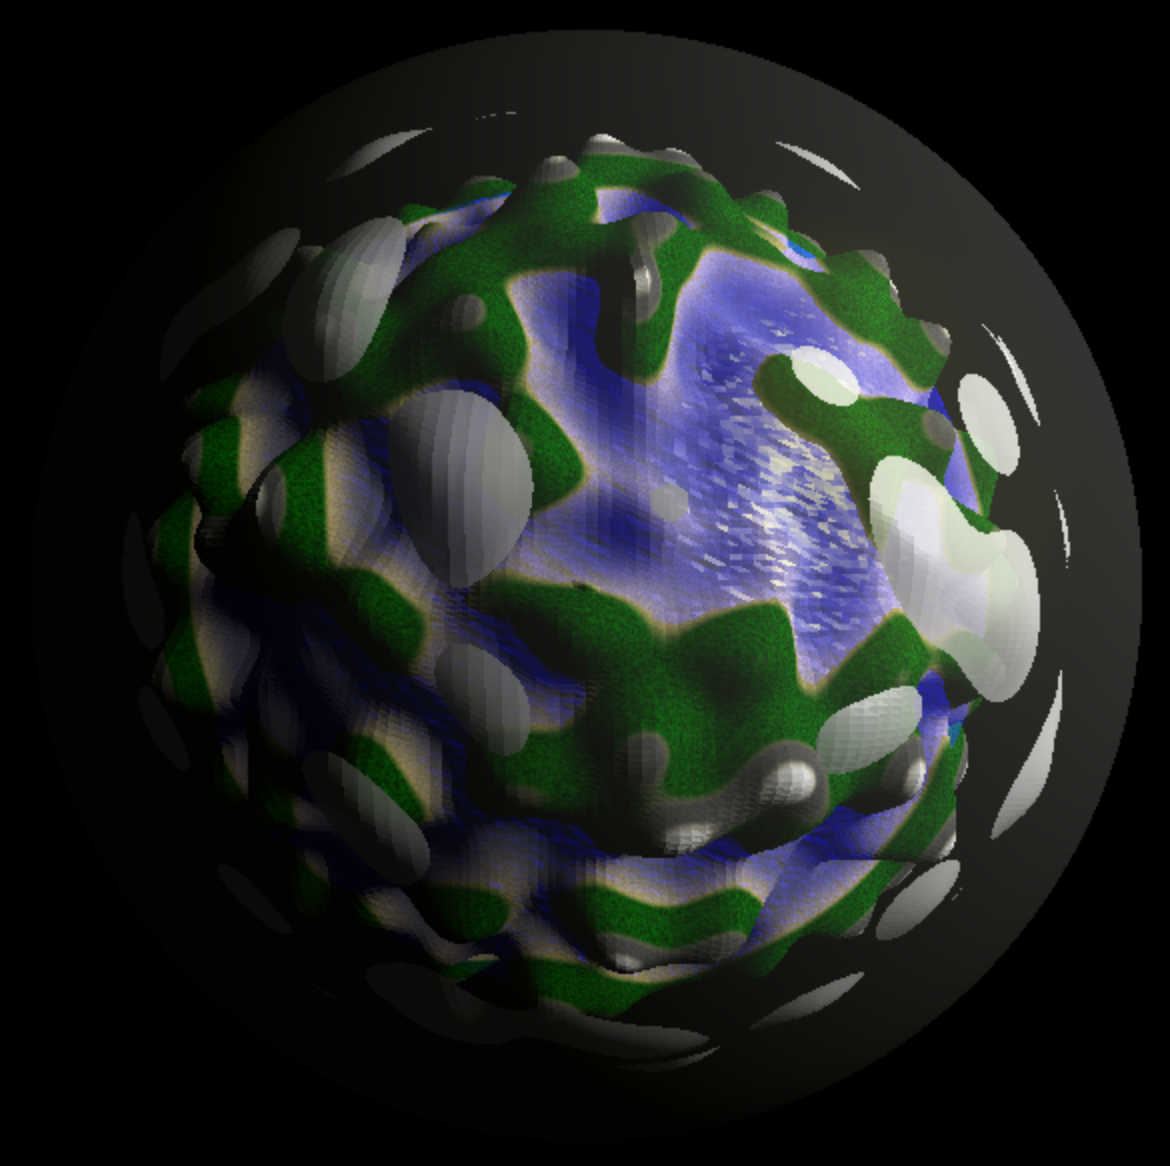
\includegraphics[width=0.8\linewidth]{./images/default}
  \captionof{figure}{Planet med standardinställningar.}\label{fig:default}
\end{Figure}

\section{Diskussion}

Det är framförallt en del av programmet som bör diskuteras, nämligen reflektionsmodellen som använts i kombination med brusfunktionerna planetens ytor. För att behålla en så hög prestanda som möjlig görs samtliga vertex-operationer på grafikkortet, i vertex-shadern. Detta leder till att punkternas normaler måste uppdateras i och med att punkterna förskjuts. Det är här shaderfunktionerna \texttt{dFdx} och \texttt{dFdy} används. Dilemmat är dock att positionerna för bildpunkterna mellan de olika vertex-punkterna interpoleras linjärt, vilket i sin tur leder till att kurvan som noise-funktionerna följer inte tas till hänsyn. Effekten av detta är att det blir tydligt synliga polygoner över ytan, se figur \ref{fig:polygons}. Detta får ytan att framstå som lågupplöst.

\begin{Figure}
  \centering
    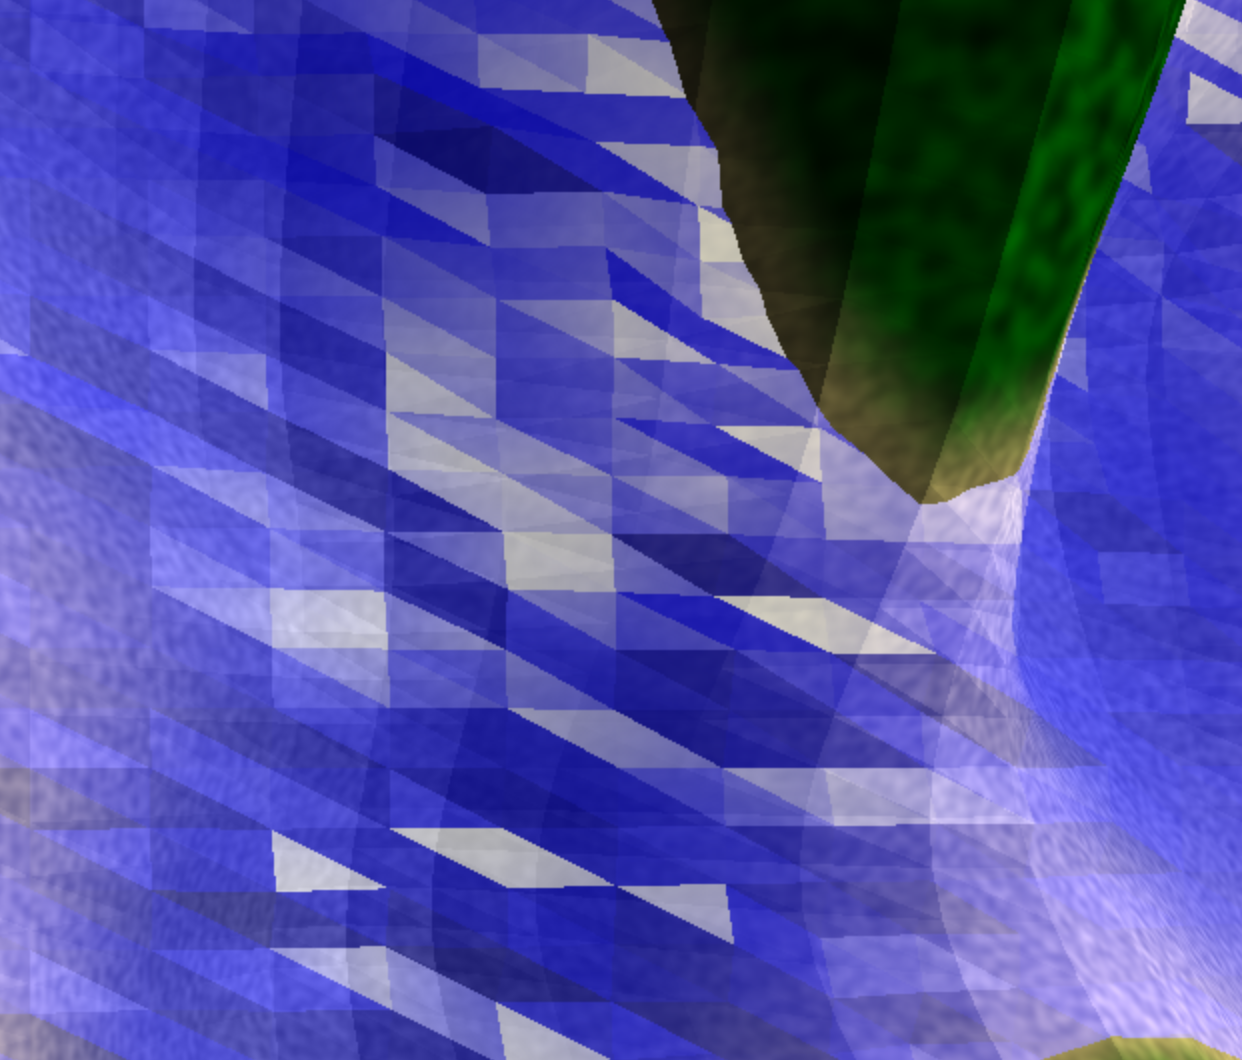
\includegraphics[width=0.9\linewidth]{./images/polygons}
  \captionof{figure}{Polygoner på vatten- och landyta.}\label{fig:polygons}
\end{Figure}

En metod för att undvika detta problem är att istället för att beräkna ytorna på CPUn direkt i programmets renderingsloop, alternativt i uppstarten av programmet om ytan inte skall gå att ändra, istället för på grafikkortet. Three.js inbyggda funktion för att räkna om normalerna skulle då kunna användas. Dilemmat med detta är att det blir en potentiell prestandaförlust, framförallt då vissa ytor använder fyrdimensionellt brus för att även animeras. En annan metod är att använda samma brusfunktion som används i vertexshadern även i fragmentshadern, och för varje bildpunkt beräkna en ny normal. Detta skulle innebära att de omkringliggande punkternas nya position även de skulle behöva beräknas. Även detta är en potentiellt dyr metod ur ett prestandaperspektiv, då en fyrdimensionell brusfunktion utför ett stort antal beräkningar och det skulle krävas två extra anrop till denna funktion - en för varje förskjuten punkt.

\begin{thebibliography}{1}

\bibitem{ref:caniuse}
  \emph{WebGL - 3D Canvas graphics}. Can I Use. Hämtad 2016-01-27. \url{http://caniuse.com/\#feat=webgl}

\bibitem{ref:stegu}
  Gustavson, S. \emph{Simplex noise demystified}. 2005, Linköping University.

\bibitem{ref:dfdx}
  Dodd, C. \emph{Explanation of dFdx}. Stack Overflow. 2013-05-03, hämtad 2016-01-27. \url{http://stackoverflow.com/a/16368768}

\end{thebibliography}

% that's all folks
\end{document}
